\documentclass[12 pt]{article}
\usepackage{amsmath,amsfonts,amssymb}
\usepackage{url}
\usepackage{graphicx}
\usepackage{setspace}
\usepackage{pgf}
\usepackage{tikz}
\usepackage{longtable}
\usetikzlibrary{arrows,automata}
\usepackage[latin1]{inputenc}
\usepackage{verbatim}
\usepackage{lscape}
%\usepackage[margin=1.2in]{geometry}

	\addtolength{\oddsidemargin}{-.5in}
	\addtolength{\evensidemargin}{-.5in}
	\addtolength{\textwidth}{0.75in}
	\addtolength{\topmargin}{-1in}
	\addtolength{\textheight}{1.75in}


\doublespacing
\begin{document}

\newcommand{\vocab}{\mathbf{v}}
\newcommand{\dtvec}{\mathbf{t}_\Delta}
\newcommand{\ctxvec}{\mathbf{t}_\text{ctx}}
\newcommand{\dt}{\Delta_t}
\newcommand{\prerror}{Pr_{error}}
\newcommand{\fvec}{\mathbf{x}}
\newcommand{\weights}{\mathbf{w}}
\newcommand{\X}{\mathbf{X}}
\section{Method}
We extracted the timestamp, author and text content for each post in each thread
from the forums. Our dataset was obtained from from \url{avsforums.com}.
\begin{description}
	\item[Previous time differences] All the time differences between posts made in the window. ($\dtvec$)
	\item[Time-based features] Day of week, Hour of day. Provides contextual information about when the post was made. ($\ctxvec$)
	
	\item[Content features (text)]
		Word frequency counts are used for this set of experiments. Using regression, we find the top $K$ variables that the actual $\dt$ depends on. Table \ref{vocab_exp} reflect the results of the experiments done with varying values of $K$.

\end{description}


\begin{table}
	\footnotesize
	\begin{centering}
	\begin{tabular}{|l|c|c|c|c|c|c|c|c|}
	\hline
	\input{vocab_exp}
	\hline
	\end{tabular}
	\caption{Experiment results: Varying vocabulary size}
	\label{vocab_exp}
\end{centering}
\end{table}

\subsection{Potential errors}
To be thorough, let us also enumerate the types of errors that a model making predictions could encounter.

The model can potentially make a prediction such that the next visit comes before the arrival of the next post. The predictions being made are the $\dt$ between the posts, rather than the visitation times, hence, it is possible for the model to make a prediciton that occurs before the current time. An erroneous prediction can also cause the crawler to come in before the next post (two, or more, visits, but nothing new fetched). Errors of this type waste bandwidth, since the crawler will make an unneccessary visit to the page.

Another type of error would have the prediction causing the next visit to come some time after a post. Since most predictions are almost never fully accurate, there will be some time between the post is made and hte page is fetched. These errors are still relatively acceptable, but the time difference between the post arriving and the visit should be minimised. The visit could also come more than one post later. Errors of this kind incur a penalty on the freshness of the data, more so than the after one post, especially if the multiple posts are far apart time-wise.


In the following experiments, the threads chosen from our extracted dataset are those with a 100 to 1000 posts. This amounted to 97 threads. The first 75\% of the thread was used as training data, while the remaining 25\% was used as test data. We used Support Vector machines for this regression task, employing a Radial Basis Function kernel as our learning algorithm. 

The SVR module from the Python library scikit-learn was used in the implementation of this experiment.


%include diagrams

\subsection{Evaluation metrics}
We use \emph{Mean Absolute Percentage Error} (MAPE), to measure the performance of the learnt model. This value is given by
\[
	\frac{1}{N}\sum^N_{i=1}\left|\frac{A_i-F_i}{A_i}\right|
\]
where $A_i$ is the actual value, and $F_i$ is the forecasted value for the instance $i$. Realistically, the model would not be able to come into contact with every possible window, since chances are it will make an error that causes %explain error in a new section (before this one) ?
it to visit a thread late, causing it to miss two posts or more. This value does not reflect how well the model will do in a real-time setting, but gives an idea of how far off the model is given a window. 

We also want to know the \emph{timeliness} of the model's visits. Yang et. al. \cite{Yang2009} has a metric for measuring this. Taking $\Delta t_i$ as the time difference between a post $i$ and it's download time, the timeliness of the algorithm is given by
\[T = \frac{1}{N} \sum^{N}_{i=1}\Delta t_i\]
A good algorithm would give a low $T$-score. However, a crawler that hits the site repeatedly performs well according to this metric. The authors account for this by setting a bandwidth (fixed number of pages per day) for each iteration of their testing. In our experimental results, we also take into account the number of page requests made in comparison to the number of posts. %ratio?

\begin{align*}
	\begin{array}{l@{\mskip\thickmuskip}l}
	Pr_{miss} &=  \dfrac{%
		\sum^{N-k}_{i=1} \left[\Theta_{ref\_hyp} (i,k)\right]%
	}{%
		\sum^{N-k}_{i=1} \left[\Delta_{ref} (i,k)\right]%
	}\\
	 & \\
	Pr_{fa} &= \dfrac{%
		\sum^{N-k}_{i=1} \left[\Psi_{ref\_hyp} (i,k)\right]%
	}{N-k}
	\end{array}
	\begin{array}{l@{\mskip\thickmuskip}l}
		\Delta_{ref}(i,k) &= \left\{ \begin{array}{l l}
				1, & \text{if }r(i,k) > 0 \\
				0, & \text{otherwise} 
		\end{array} \right.\\
		\Theta_{ref\_hyp}(i,k) &= \left\{ \begin{array}{l l}
				1, & \text{if ends with post} \\
				0, & \text{otherwise} 
		\end{array} \right.\\
		\Psi_{ref\_hyp}(i,k) &= \left\{ \begin{array}{l l}
				1, & \text{if ends with visit}\\
				0, & \text{otherwise} 
		\end{array} \right.\\
	\end{array}
\end{align*}
Split the $Pr_{error}$ measure into 3 parts:

Probability of having visits before the first post in the window.
Probability of having more visits than posts after the first post.
Probability of having more posts than visits after the first post.



Viewing the posts made during the thread's lifetime as segmentations of the thread, and the visits made as hypotheses of where the segmentations are, we use the $\prerror$ metric from Georgescul et. al., 2006 as a measure of how close the predictions are to the actual posts. An example can be seen in Figure \ref{prerror}.



Function that gives me:

Increase in visit to post ratio		increase
Increase in interval				increase

Increase between post and visit		increase
(0,$\infty$ or 1)

Increase between visit and visit	decrease
($\infty$ or 1,0)
Increase between post and post		increase
(0,$\infty$ or 1)

\[
	\begin{array}{l l}
	T = \dfrac{%
		\sum_{e=1}^{|E|-1} \Psi(e_t,e_{t+1}) %
	}{|E|-1} &
		\Psi(e_t,e_{t+1}) = \left\{\begin{array}{l l}
				1-e^{-(e_{t+1} - e_t)}	& \text{if post,visit}\\
				e^{-(e_{t+1} - e_t)}			& \text{if visit,visit}\\
		\end{array}\right.
\end{array}
\]

\begin{figure}
\[
	\uparrow~~p_1,\underbrace{~~p_2,~~p_3,~~~p_4,\uparrow}_{\text{sliding window}}\uparrow
\]
\caption{An example of the sliding window metric. The metric is made up of two components: First, the probability that, given at least one post is present in the window, there are more visits than post. Secondly, the probability that there are more posts than visits for a given window. The weighted sum of this gives the overall $\prerror$}\label{prerror}
\end{figure}

\section{Results}

The results for experiments done with different combinations of the above specified features are shown in Table \ref{expt1}.
\begin{table}
	\footnotesize
	\begin{centering}
	\begin{tabular}{|l|c|c|c|c|c|c|c|}
	\hline
	\input{init_res}
	\hline
	\end{tabular}
	\caption{Experiment results}
	\label{expt1}
\end{centering}
\end{table}
\begin{centering}
\tiny
	\begin{longtable}{|l|c|c|c|c|c|c|}
	\caption{Experiment results}
	\input{usernameresults}
	\end{longtable}
	\label{username}
\end{centering}


Overall average and window average perform significantly worst than the learnt models, as reflected in both the MAPE and the $T$-score. There is also a slight improvement in the  $\prerror$ in the learnt models.


Taking into account the $T$-score and the number of visits together, would seem that $\dtvec$, features representing the previous time intervals, are important features when determining the next time interval. In the absence of these features, we observe that the $T$-score increases by about 1\%. In this experiment, we use purely word frequency features. This gives only a slight improvent over not using them.

High values for $Pr_{miss}$ and low for $Pr_{fa}$, are due to $Pr_{miss}$ being conditioned on there being a post within the window. Since the posts come in bursts, visits are fairly periodic, and intervals between visits are larger than post bursts. When there are more posts than visits in windows with posts, we have higher $Pr_{miss}$

\begin{landscape}
\begin{figure}
	\centering
	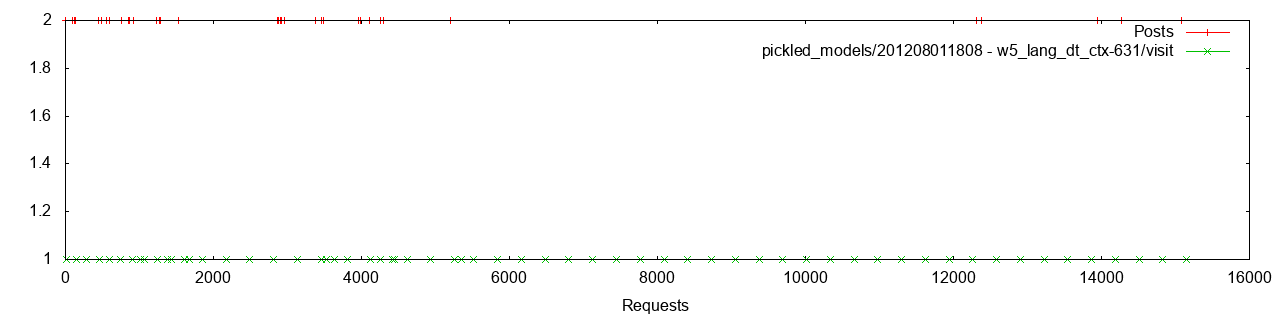
\includegraphics[scale=0.5]{example_seq.png}
	\caption{Visitation chart for a model using the $w=5, \mathbf{t}_\Delta, \mathbf{t}_{\text{ctx}},\mathbf{w}$ feature set. Invalid Predictions = 0.758, $Pr_{error} =  0.485$, $T$-score = 119.612, Posts = 41, Visits = 62}
\end{figure}
\end{landscape}

\begin{table}
	\footnotesize
	\begin{centering}
	\begin{tabular}{|l|c|c|c|c|c|c|c|c|}
	\hline
	\input{f_size}
	\hline
	\end{tabular}
	\caption{Experiment results: Varying feature sizes}
	\label{exp_f_size}
\end{centering}
\end{table}

\begin{table}
	\footnotesize
	\begin{centering}
	\begin{tabular}{|l|c|c|c|c|c|c|c|c|}
	\hline
	\input{f_size_ebackoff}
	\hline
	\end{tabular}
	\caption{Experiment results: Using exponential increase}
	\label{exp_exp}
\end{centering}
\end{table}

\subsection{Discounted sum of previous instances}

The current method uses only information on the current $w$ posts. However, posts made further in the history of the thread may have an effect on when the latest posts arrive. The magnitude of this effect, however, may diminish over time.

Following this intuition we attempt to use a discounted sum over previous posts' word frequency vector:
\[
	\fvec_t = \vocab_t + \alpha \fvec_{t-1}
\]
where $\fvec_t$ is the feature vector at post $t$, and $\vocab$ is the word frequency vector. $\alpha$ is the \emph{discount factor} and satisfies $0 \leq \alpha < 1$.


\begin{table}
	\footnotesize
	\begin{centering}
	\begin{tabular}{|l|c|c|c|c|c|c|c|c|}
	\hline
	\input{decay_w15}
	\hline
	\end{tabular}
	\caption{Experiment results: Window size of 15, using discounted sum feature vector at $t-1$.}
	\label{exp_decay}
\end{centering}
\end{table}

\subsection{Stochastic Gradient Descent}

We attempt to use stochastic gradient descent to estimate the function $f$. However, during runtime, instead of using a static function, we continue to allow $f$ to vary whenever new posts and their update times are observed.
Since $f(\fvec_{t-w},\hdots,\fvec_{t-1}) > 0$, we used a scaled sigmoid function,
\[
	f(\X) = \frac{\Lambda-\lambda}{1 + e^{\weights \cdot \X}} + \lambda
\]
where $\Lambda$ and $\lambda$ are the scaling factors. This results in $f: \mathbb{R}^{|\X|}  \rightarrow (\lambda,\Lambda)$. Bounding the estimation function between $\lambda$ and $\Lambda$ allows us to restrict the prediction from becoming negative, or, becoming exceedingly huge. For our purposes, we set $\lambda = Q_3 + 2.5(Q_{3} - Q_{1})$, where $Q_n$ is the value at the $n$-th quartile. 

The resulting update rule for $\weights$ is then given by,
\[
	\Delta \weights_i = \eta
				\underbrace{\left(\widehat{\dt} - \dt \right)}_{\text{error term}}
				\underbrace{\left( f(\X)(1-f(\X)) \right)}_{\text{gradient}}
						\X_i
\]
which is similar to the delta update rule found in artificial neural networks. We omit the scaling factor in the gradient as it is a constant and then experiment with various values of $\eta$, the learning rate. The results are seen in Table \ref{sig_grad_desc}
\begin{table}
	\footnotesize
	\begin{centering}
	\begin{tabular}{|l|c|c|c|c|c|c|c|c|}
	\hline
	\input{sig_grad_desc}
	\hline
	\end{tabular}
	\caption{Experiment results: Using stochastic gradient descent, with $\lambda = 0$}
	\label{sig_grad_desc}
\end{centering}
\end{table}

\bibliographystyle{acm}
\bibliography{report}
\end{document}
